\chapter{Statistical Connectomics} \label{chap:chap-3}

This chapter documents our first investigation into the alpha blocker treatment hypothesis in humans facing a severe respiratory illness. Importantly, this study leveraged large insurance claims databases and common health conditions during a period where the COVID-19 data environment was too immature to produce a sufficiently large and well-understood sample for this analysis. This chapter was originally published in Annual Review of Statistics and Its Application in March 2021 (DOI: \burl{https://doi.org/10.1146/annurev-statistics-042720-023234}) and is distributed under the terms of a Creative Commons Attribution License that permits unrestricted use and redistribution provided that the original author and source are credited.

\pagebreak
\section*{Abstract}
The data science of networks is a rapidly developing field with myriad applications.  In neuroscience, the brain is commonly modeled as a connectome, a network of nodes connected by edges. While there have been thousands of papers on connectomics, the statistics of networks remains limited and poorly understood.  Here, we provide an overview from the perspective of statistical network science of the kinds of models, assumptions, problems, and applications that are theoretically and empirically justified for analysis of connectome data.  We hope this review spurs further development and application of statistically grounded methods in connectomics.
\pagebreak

\section{Introduction}
The idea of the brain as a network of interconnected neuronal elements has existed since the late 19th century. These neuronal elements (e.g. long-range fibers, synapses, subcellular processes) are anatomically organized in multiple scales of space to allow communications over multiple scales of time enabling perception, cognition and action \citep{Shepherd1991-ri,Rieke1997-ok,Russell2016-gt}. Recent advances in neuroimaging \citep{Chung2013-zb,Hagmann2005,Biswal2010-hk} along with large-scale projects opened new frameworks for studying the brain by modeling  brain connectivity as networks, or connectomes \citep{hcp1,zuo2014open,alexander2017open}. One of the main challenges in connectomics is to understand the network structures that link individual histories, such as the genome, developmental stage, or experience, to cognitive phenotypes, such as personality traits, behaviors, or disorders, which has been dubbed ``connectal coding''~\cite{vogelstein2019connectal}.

A connectome is defined as an abstract mathematical model of brain structure as a network, composed of two sets: vertices (or nodes) that represents a biophysical entity of the brain, and edges that represent connections, or communication, between pairs of vertices \citep{sporns2005human,Hagmann2005,vogelstein2019connectal}. Connectomes can have additional structures. For example, edges can have weights that describe the strength of connection, and have other attributes, such as physical location of the edge. Similarly, nodes can also have attributes, such as anatomical labels, shape and size. This capacity of connectomes as a brain model comes with challenges in their analysis. 

The first challenge is the choice of the representation of a connectome. Figure \ref{fig:intro_fig}a and \ref{fig:intro_fig}b shows two valid, but different representations of a human connectome. In Figure \ref{fig:intro_fig}a, the connectome is shown as a collection of vertices and edges in the classical graph theory perspective.
The vertices are organized by their location in the human brain, but this is only one choice of layout. There are infinitely many layouts that are equally valid, and, potentially, useful.
In Figure \ref{fig:intro_fig}b, the connectome is shown as a collection of numbers laid out in rows and columns as an ``adjacency matrix'' in the computer science perspective. In this view, a row/column pair is a vertex, and edges between vertices $u$ and $v$ are depicted by a non-zero entry in the corresponding element of the matrix. Consequently, the row identities are linked to column identities. Permuting both rows and columns together results in a ``different'' matrix, but they represent the same connectome. Nonetheless, the adjacency matrix is a useful representation of connectomes.

The second challenge is that connectomics data are different from typical Euclidean data in many ways. Some operations, such as addition and multiplication, are not well defined. What would it mean to add two connectomes together? Distance metrics are also not well defined, making comparisons between connectomes difficult. In the view of adjacency matrices, each entry is potentially related and dependent on other entries.

The third challenge is that connectomics data can be highly variable. For a graph with $n$ vertices, there are $n \choose 2$ possible edges so the number of unique graphs is $2^{n \choose 2}$. Figure \ref{fig:intro_fig}c shows the exponential growth in the number of unique graphs as the number of vertices increase. The large number of possible graphs makes characterizing and describing the graphs is difficult without statistical analysis of connectomics data.
% TODONE a third challege, there are many, eg, 2^n^2 of them with n vertices.  maybe worth showing that sequence in fig 1? maybe also for unlabeled? that there are so many means that we will really need statistics. 

Current connectomics analysis frameworks can be organized into four categories, each of which address the above challenges to various extents.
The first approach, and by far the most popular, is dubbed the bag of features. In this approach, a set of graph-wise or vertex-wise statistics that capture the structural aspects of networks are computed and compared \citep{Bullmore2010-ew,mhembere2013computing}. One major drawback to this method is that features are not independent of one another, making results from subsequent inference using these features difficult to interpret.
In the second approach, the bag of edges, each edge is studied individually. As a consequence, edges are treated independently, ignoring the other potential interactions \citep{Craddock2013-qs,Varoquaux2010-tc}. 
In the third approach, the bag of vertices, the vertices are studied while leveraging some structural information of the connectomes.
In the fourth approach, the bag of communities, the vertices are first organized into (typically) disjoint groups to form communities, and then edges within and across communities are studied. The last approach, the bag of networks, studies the connectomes as a whole to test for differences across groups or to classify connectomes.

While each of the frameworks provide complementary and meaningful insights into the connectomes, the underlying methodologies, and, thus, the interpretation of results can vary significantly. Statistical modeling of connectomes bridges the gap by providing a unified framework for studying connectomes. Conceptually, statistical models capture important differences within or among networks while considering the built-in structures and heterogeneity in networks \citep{Zheng2009-df,athreya2017statistical,arroyo2019inference, zhang2018network}. These differences are summarized by model parameters that can be used in a variety of subsequent inference tasks. 

This article is intended as a quantitative review of current connectomics analysis methods, and how statistical models can be incorporated to improve current analysis methods. We perform empirical investigations to demonstrate to what extent conclusions can be trusted as a function of the analysis method and the hypothesis in consideration. We vary parameters for the data, such as the generative model, sample size, and effect size, and hypothesis testing frameworks. Ultimately, the statistical modeling of networks uniquely provides a framework for meaningful and accurate testing and estimation for connectomics.

\begin{figure}
    \centering
    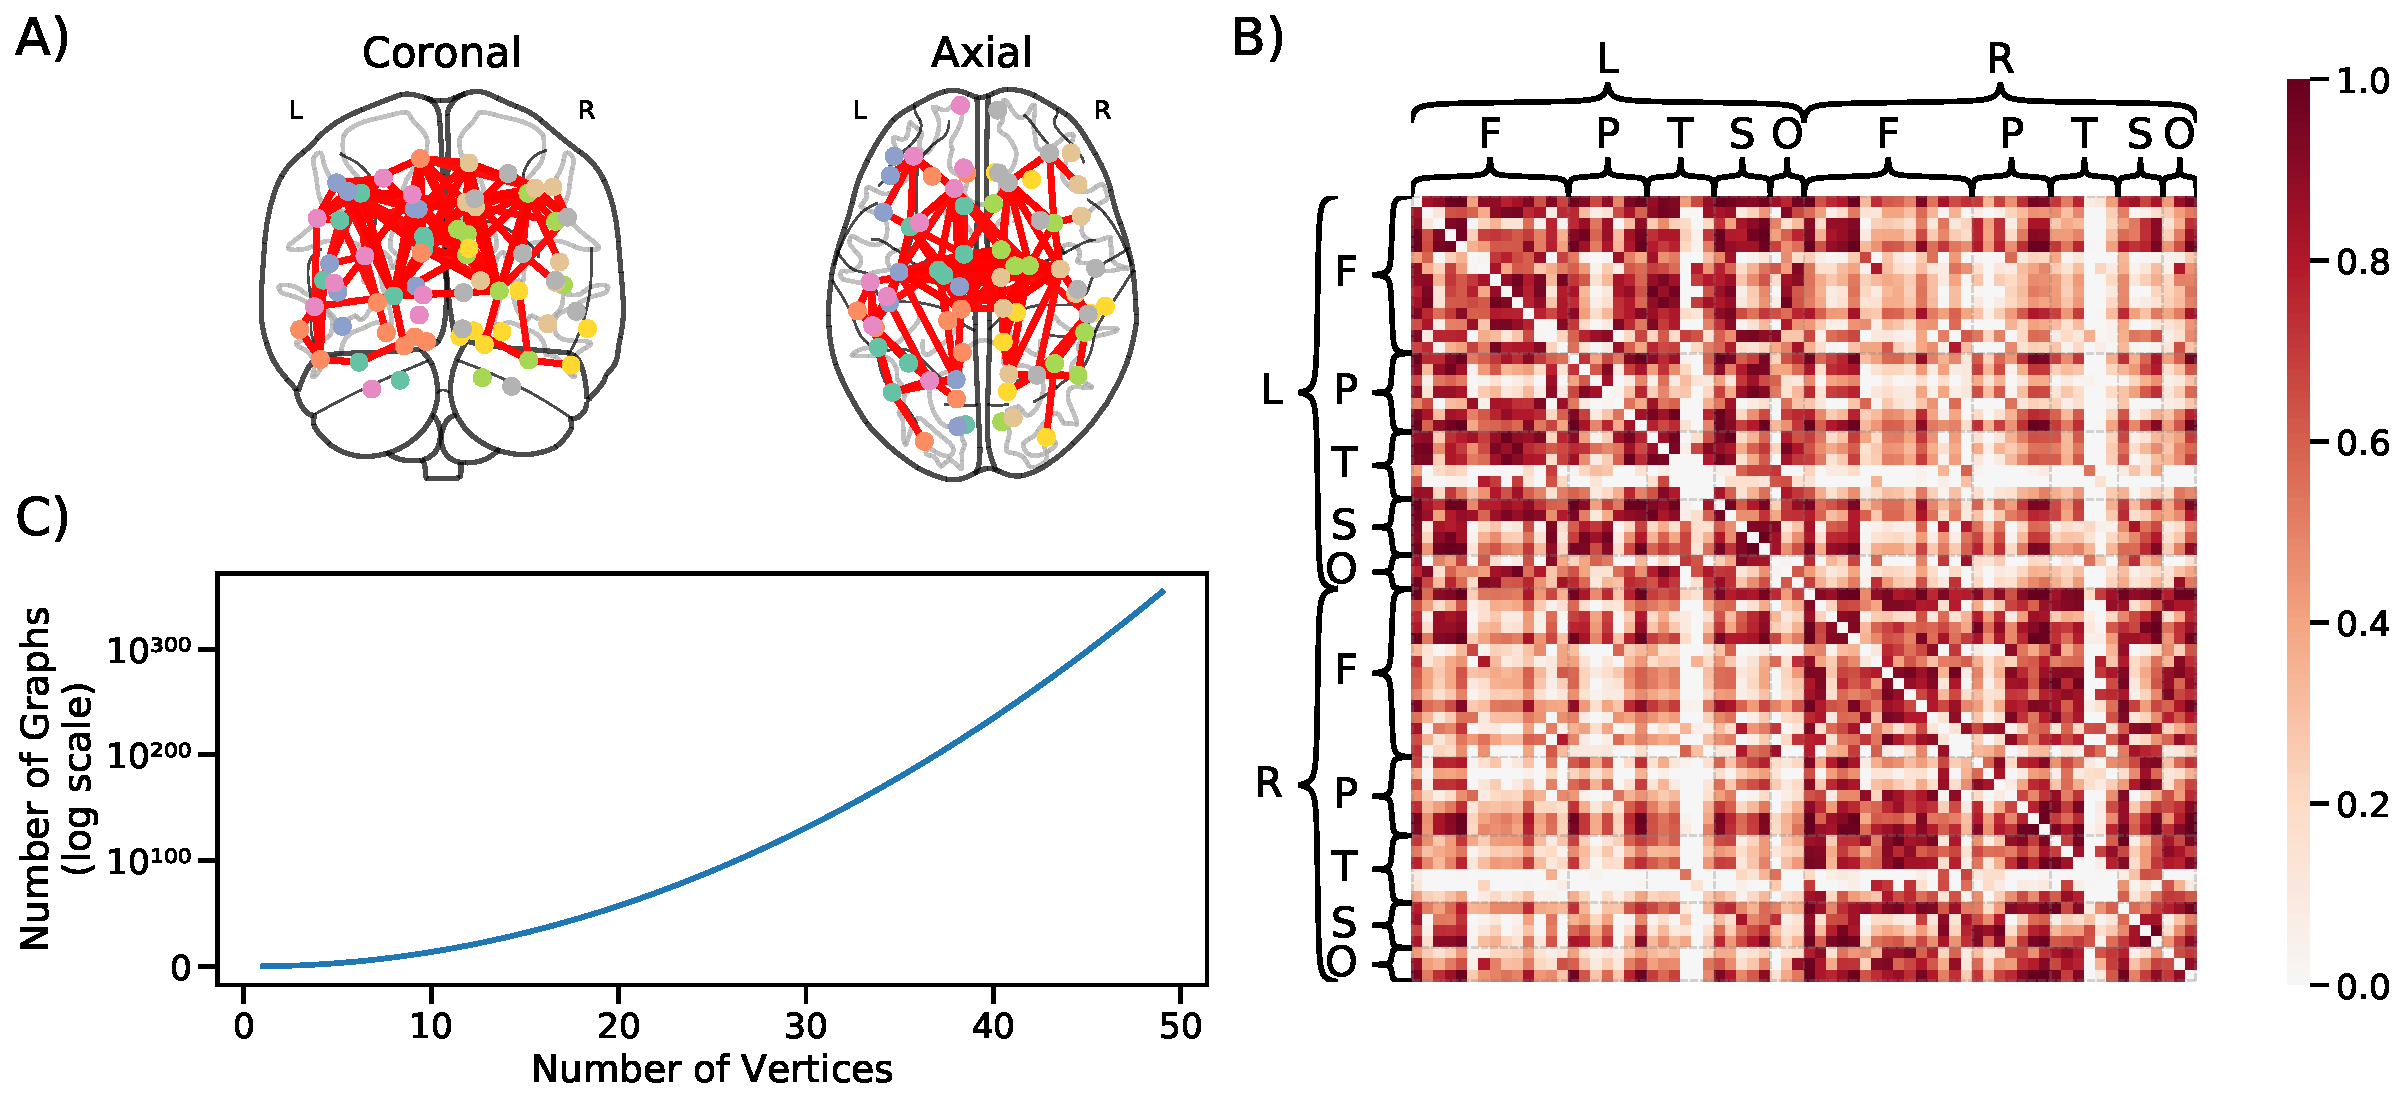
\includegraphics[width=\textwidth]{figures/dnd/intro}
    \caption{
    \textbf{Different Representations of a Connectome.} 
    Human structural connectome estimated from averaging 1059 human connectomes from the Human Connectome Project \citep{hcp1}.
    Vertices represent regions of the brain, and are assigned into right (R) and left (L) hemispheres and then further assigned into frontal (F), occipital (O), parietal (P), and temporal (T), and subcortical structures (S). 
    \textbf{a.} Connectivity shown in the coronal and axial views. Dots corresponds to the center-of-mass of the a region, lines correspond to connections, and line thickness corresponds to magnitude of the connection. Only the largest 5\% of edges are shown for visualization purposes. Note that infinitely many spatial arrangement of the vertices exist, and only one particular arrangement is being shown.
    \textbf{b.} Connectivity of the average structural connectome shown as an adjacency matrix, $\A$. The rows and columns are organized by hemisphere then further organized by sub-structures. However, given any permutation matrix $\Pbf$, the permuted adjacency matrix $\Pbf\A\Pbf^\top$ is still a valid matrix of original connectome. For a graph with $n$ vertices, there are $n^2$ permutations.
    \textbf{c.} The number of unique graphs grows exponentially as the number of vertices increases. The large number of graphs motivate statistical analysis to characterize and describe connectomes.
    } 
    \label{fig:intro_fig}
\end{figure}


\section{Representations}\label{sec:representations}
Due to the flexibility of networks, different representations of the connectomes can be studied, which we organize into four categories. In the following sections, we first formally define a network and then describe the four different frameworks of studying connectomics data. All frameworks provide complementary insights and understanding of the connectomes. 

\subsection{Graph/Network}
\label{sec:unwt_graph}
A graph, or network, $\mathcal{G}$, is defined as an ordered set of vertices and edges $(V, E)$ where $V$ is the vertex set, and $E$, the set of edges, is a subset of the Cartesian product of $V \times V$. That is, a graph has at most a single edge for each pair of unique vertices. A vertex set is represented as $V=\{1, 2, \ldots, n\}$ where $|V| = n$, and an edge exists between vertices $i$ and $j$ if $(i, j)\in E$. An unweighted graph is a graph in which we are only concerned with the presence (or absence) of an edge. Each graph has an associated adjacency matrix $\A \in \left\{0, 1\right\}^{n\times n}$ where $\A_{ij}$ represents the presence (or absence) of the edge between nodes $i$ and $j$. Note that $\A$ provides a unique representation of $\mathcal{G}$; that is, there exists a $1$-to-$1$ relationship between a graph and its adjacency matrix. 

The above definition can be further extended in two ways: 
\begin{enumerate}
    \item Weighted graphs - the edges can take on arbitrary values, typically a real number. For example, the edge weight in human structural connectomes are non-negative integers that represent the number of estimated neuronal fibers that traverse from one region of the brain to another. Thus, each weighted graph has an adjacency matrix $\A\in\RR^{n \times n}$ where $\A_{ij}$ represents the edge weight.
    \item Directed graphs - $E$ is now an \textit{ordered} set of edges. Each edge has an associated direction, and a directed edge exists between vertices $i$ and $j$ if $(i,j)\in E$. In undirected graphs, the associated adjacency matrix $\A$ is symmetric, but in directed graphs, $\A$ is not necessarily symmetric, that is, it is possible that $\A_{ij}\neq\A_{ji}$, for any $i, j\in V$.
\end{enumerate}

For the remainder of the paper, graphs are considered undirected and unweighted and with no self-loops, that is $\text{diag}(\A) = \Vec{0}$, unless specified otherwise.

\subsection{Bag of Features}\label{sec:bag-of-features}
Network statistics, or features, are abstract representations that capture either global or local structures of a network \citep{priebe_coppersmith_rukhin_2010,mhembere2013computing}. This method computes a set of network statistics for each network, and analyzes differences between, or among, populations. For example, when comparing populations of networks from healthy and individuals with depression, the difference in global clustering coefficient, which measures how likely vertices tend to cluster together, can be computed \citep{Bullmore2009-yj}. These network statistics have enjoyed applications in many connectomics studies that compare different populations of networks \citep{bullmore2011brain, ghoshdastidar2017two}. However, there are infinitely number of such statistics, and we lack general guidance in which statistics to compute. Furthermore, no set of network statistics can adequately characterize a network \citep{chen2018same,matejka2017same}. These considerable shortcomings further motivates the use of other representations of networks, and below examples demonstrate the shortcomings of studying bags of features.

\subsubsection{Non-identifiability of graph features}
Summary statistics, such as the mean, variance, and correlation, are often used to describe real valued datasets, which can be insightful in understanding the data. However, the Anscombe's quartet illustrates four drastically different distributions of eleven points that have the same summary statistics \citep{anscombe1973graphs}. This suggest that any small number of summary statistics can fail to meaningfully characterize the data. 

In network analysis, variety of network level statistics can be computed to summarize networks. Similar to the Anscombe's quartet, networks with different topologies can have the same network features as shown in Figure \ref{fig:exp5}. These four networks have the same number of vertices, edges, triangles, and global clustering coefficient, but have different properties such as connectedness and symmetry. Other works have also explored the distributions of network statistics \citep{chen2018same,matejka2017same}. 

\begin{figure}
    \centering
    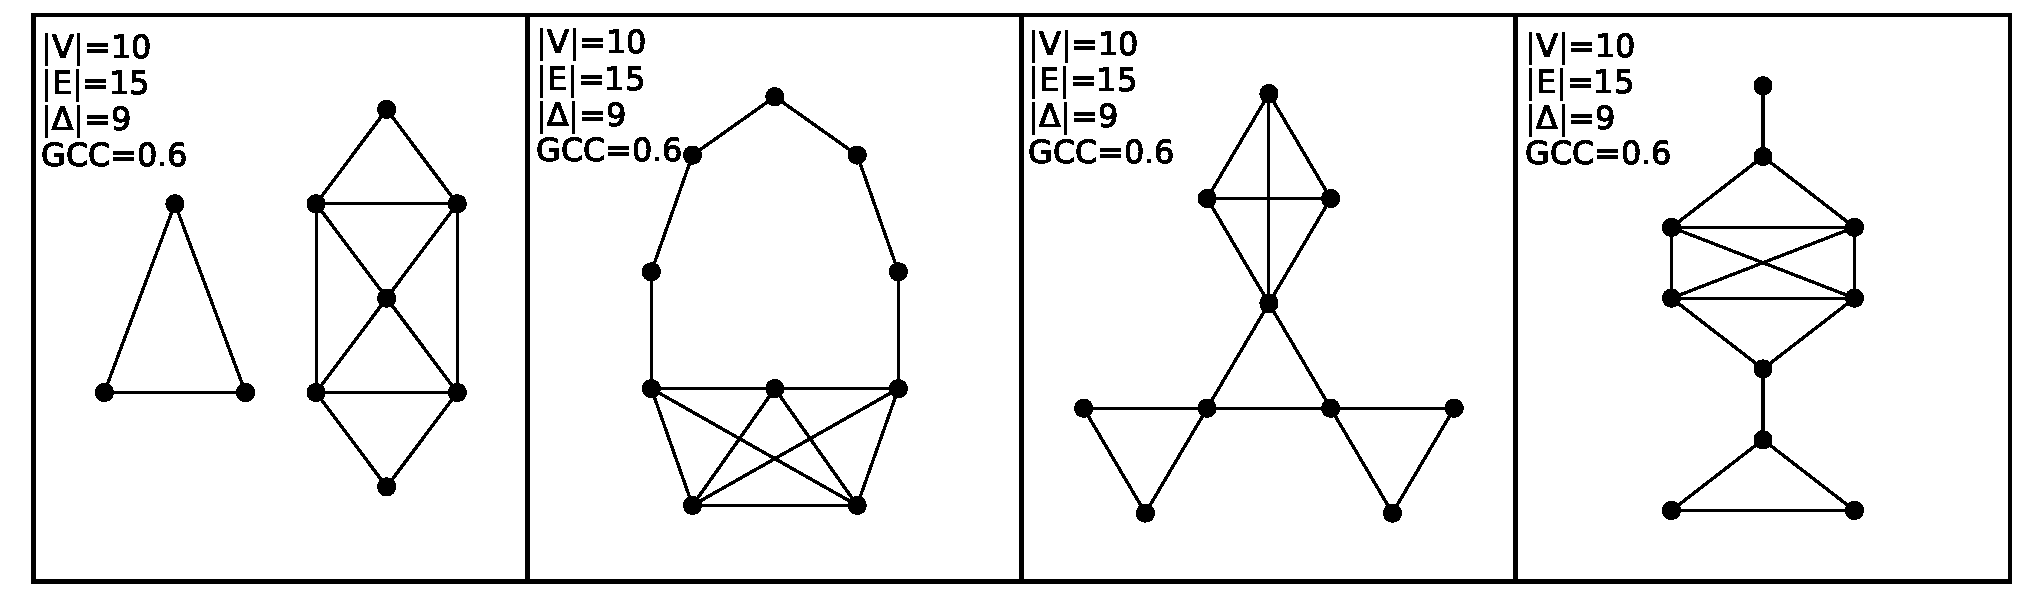
\includegraphics[width=.9\textwidth]{figures/dnd/exp5_10nodes_row}
    \caption{
    \textbf{Four Networks with Same Network Statistics.} Each network has 10 vertices ($\abs{V}$), 15 edges ($\abs{E}$), 9 triangles ($\abs{\Delta}$), and the global clustering coefficient (GCC) is 0.6. However these graphs have distinctive topologies. For example, the left-most network is disconnected, while others are connected. This suggest that given a small set of network statistics, one cannot identify from which network the features are computed.
    }
    \label{fig:exp5}
\end{figure}

\subsubsection{Network features are correlated and relatively uninformative}
We consider all non-isomorphic, undirected, binary networks with 10 vertices, which results in $\approx12$ million networks. Formally, $\mathcal{G}$ and $\mathcal{H}$ are isomorphic networks when there exists a vertex permutation function $f:V(\mathcal{G})\rightarrow V(\mathcal{H})$ such that if edge $(u,v)\in E(\mathcal{G})$, then $(f(u), f(v))\in E(\mathcal{H})$. Only non-isomorphic networks are considered since isomorphic networks have identical network features.

For each network, the following six graph network statistics are computed: 1) average path length (APL), 2) global clustering coefficient (GCC), 3) average clustering coefficient (ACC), 4) global efficiency (GE), 5) local efficiency (LE), and 6) modularity. These statistics are some of the most commonly computed statistics \citep{sporns2005human,Bullmore2009-yj}. The distribution of network statistics are plotted against modularity. 
The top row of Figure \ref{fig:exp6} shows that all of the network features are highly correlated with modularity.
We then constrain the networks in two different ways. First, we consider all networks with $20 \pm 2$ edges. Second, we choose a ``base'' network at random with 20 edges, and then identify all networks with no more than 3 edges different from the  base network. The distribution of each of the above network statistics on this subset of networks are computed for both constraints. The middle and bottom rows of Figure \ref{fig:exp6} show that constraining the networks in these ways hardly constrains the network features at all. Similar pattern is shown in the analysis of HCP data as shown in Supplemental Appendix \ref{sec:bag-of-features-hcp}. Changing only a few edges on a network can yield a network with almost any possible configuration according to these statistics, and therefore are inadequate to characterize these populations. Thus, when any given metric is correlated with a covariate of interest, so are many other metrics. Thus, claiming that a particular property of the brain ``explains'' a given phenotypic property of a person is spurious reasoning.

\begin{figure} 
    \centering
    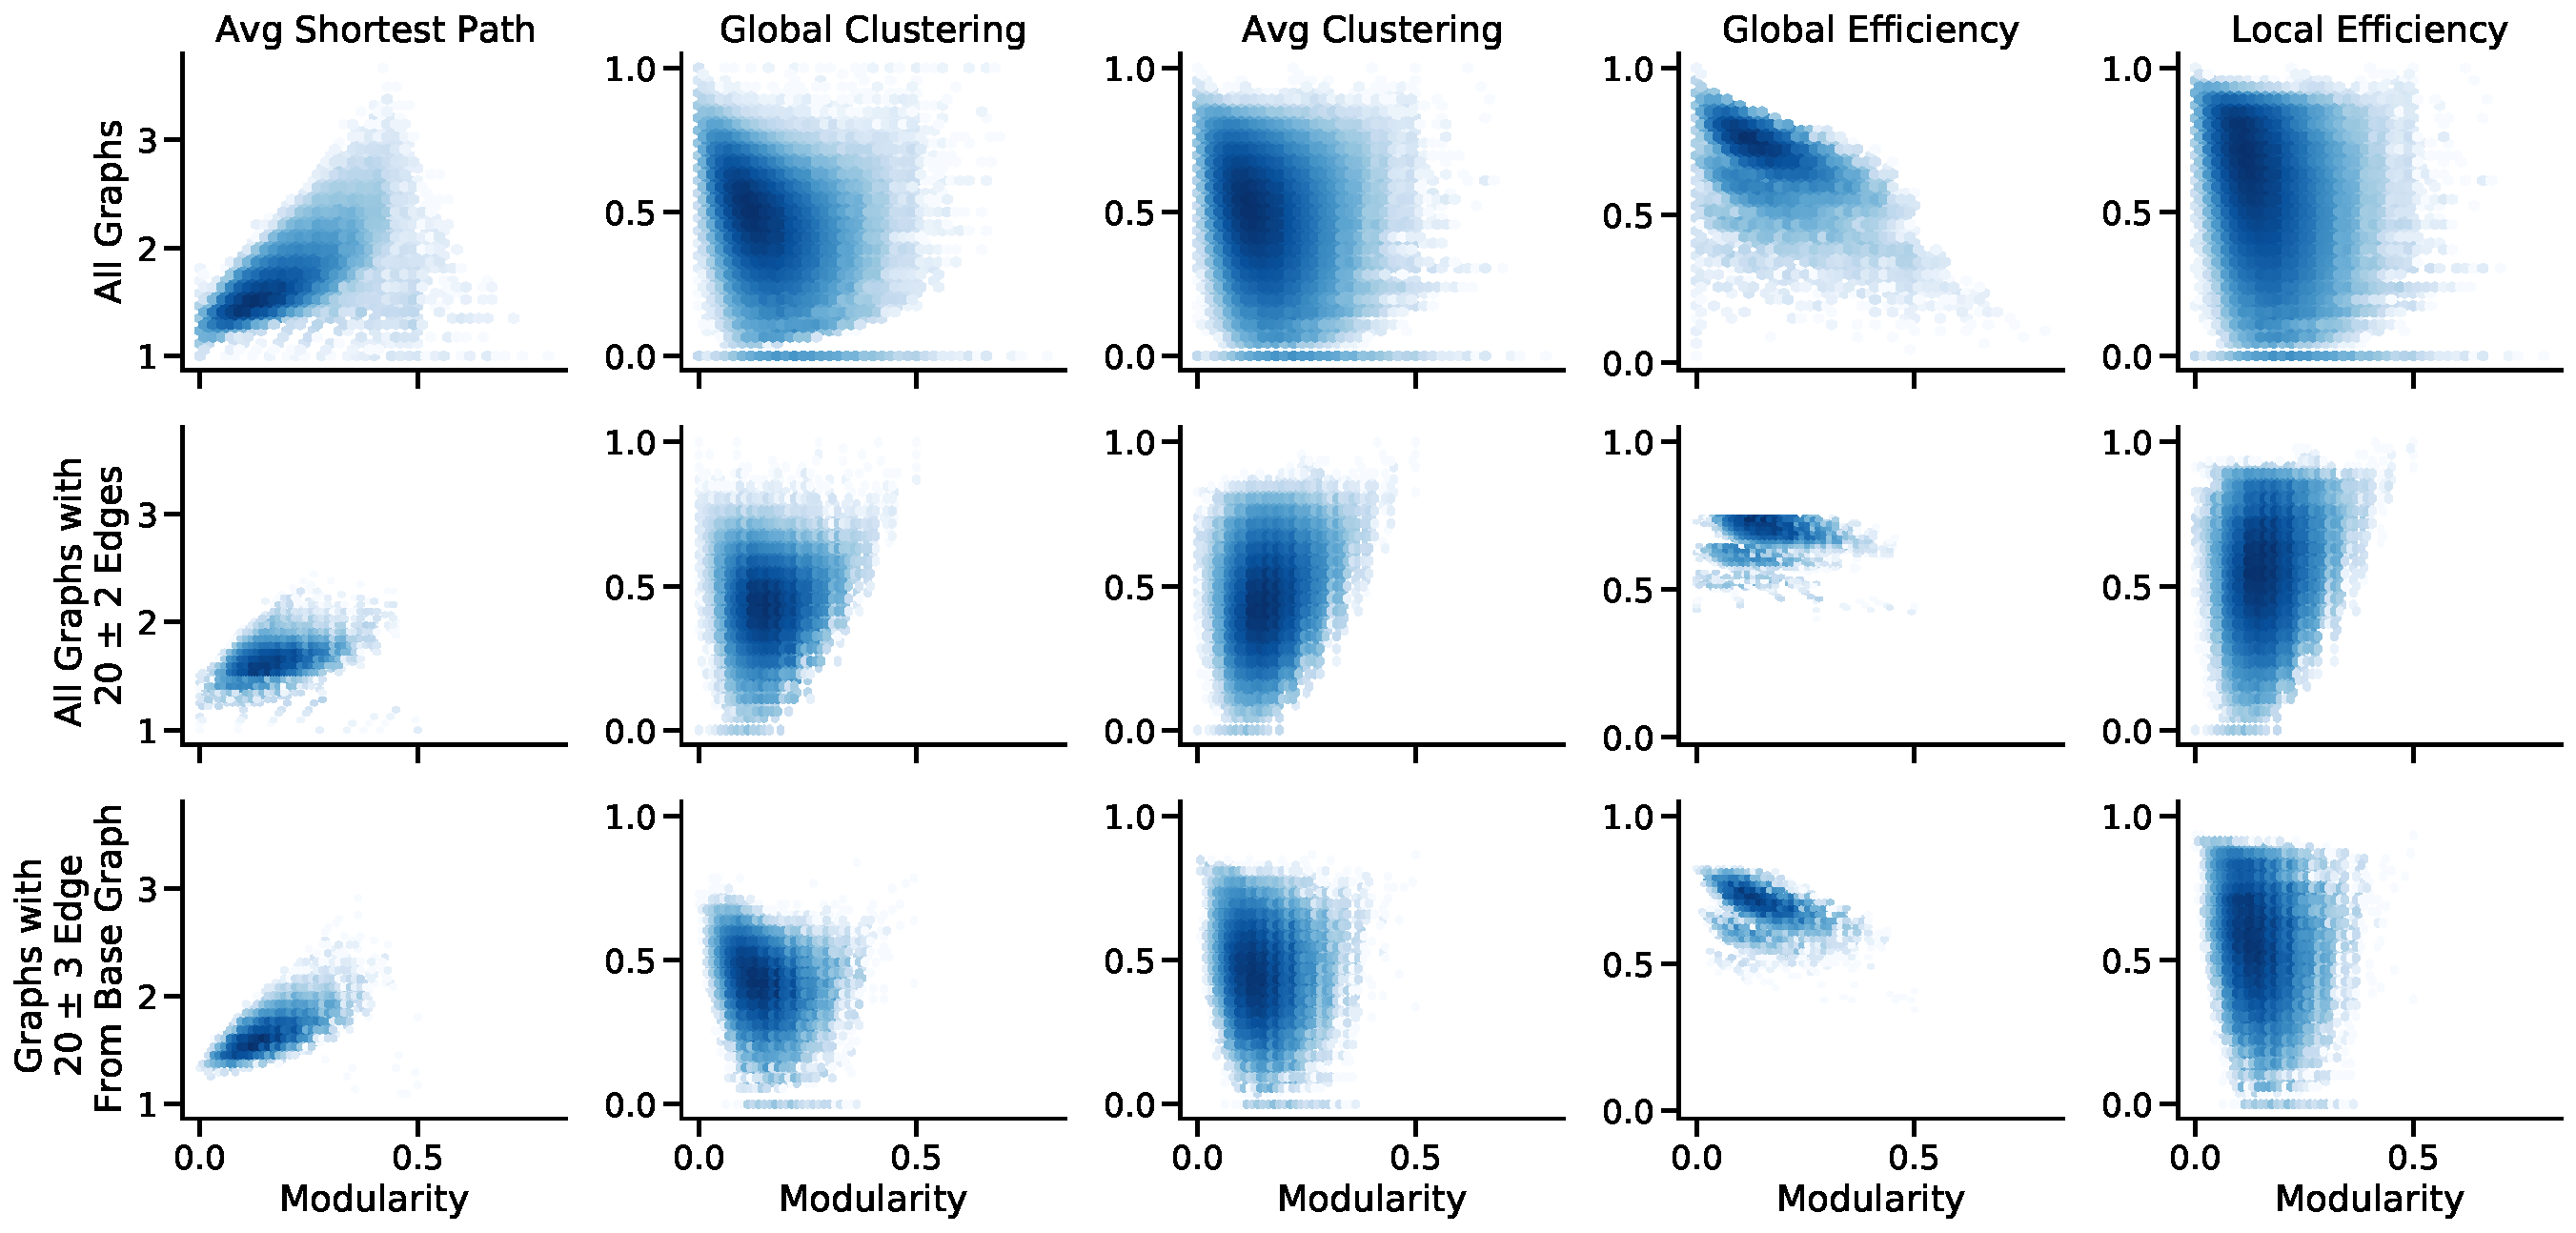
\includegraphics[width=\textwidth]{figures/dnd/density_num_edge_20_row}
    \caption{\textbf{Density plots of network statistics.} \textit{(Top Row)} The distributions of networks statistics for all possible 10-node networks are shown. \textit{(Middle Row)} Networks are constrained by only considering all networks with $20 \pm 2$ edges. \textit{(Bottom Row)} A base graph with $20$ edges is chosen at random, and only networks that have differences up to $3$ edges are considered. In both constrained set of networks, the distribution of these network statistics remains essentially unchanged. In other words, changing only a few edges on a network can yield a network with almost any possible configuration according to these statistics. }
    \label{fig:exp6}
\end{figure}

\subsection{Bag of Edges}\label{sec:bag_of_edges}
In this approach, the edges of connectomes are studied. Most commonly, each edge is studied independently, while ignoring any interactions between edges \citep{Craddock2013-qs,Varoquaux2013-hy,zhang2018mapping}. Univariate edge-wise testing can reveal easily interpretable relationships between specific edges and covariates through hypothesis testing. However, edge-wise testing requires performing multiple hypothesis tests, and multiple comparisons must be corrected to control the false positive rate \citep{Genovese2002-yq,Efron2008-zq}. While certain methods, such as Benjamini–Hochberg corrections, have strong theoretical guarantees, they require assumptions about the data, such as independence, that connectomics data do not satisfy \citep{Zalesky2010-ox,Benjamini1995-ij,Simes1986-gn}. On the other hand, Bonferroni corrections are considered too conservative, and, therefore, lack the sensitivity for connectomics \citep{Simes1986-gn}.

More intricate methods represent each connectome as a long vector containing all of its edges \citep{richiardi2011decoding, amico2017mapping}. Vector representations can allow for correlation of edges and direct application of common machine learning algorithms, but still discards the structural information in networks.

\subsection{Bag of Vertices}\label{sec:bag_of_nodes}
In this approach, the vertices of connectomes are analyzed while leveraging structural information, typically global structures, of the graphs. 
A common approach embeds the connectomes to learn a low-dimensional and Euclidean representation of the vertices \citep{grover2016node2vec, athreya2017statistical, arroyo2019inference}. Algorithms that operate on Euclidean data (e.g. Gaussian Mixture Model ($\gmm$) for clustering vertices, random forests for classifying vertices, multivariate hypothesis tests for testing for differences between vertices) can be employed for subsequent analysis \citep{priebe2017semiparametric, tang2018connectome}. 

\subsection{Bag of Communities}
Networks often contain structural information such as communities, which are subsets of vertices that behave similarly. For example, similar vertices can be defined by those that are more likely to be connected with each other than to other vertices.
The set of communities that comprise a network, called community structure, can describe both the local and global patterns of the network. At local-scale, we can examine the properties of vertices that are within the same community. At global-scale, we can measure associations between connectivity patterns of communities across groups or other covariates \citep{faskowitz2018weighted, kim2019graph, arroyo2020simultaneous}. Furthermore, the community structure in spatial resolution connectomes from human MRI can be used to delineate regions of the brain, called parcellations \citep{thirion2014fmri}.

Community detection in networks have been studied extensively \citep{newman2013spectral, fortunato2016community}. Typically, the community structure is identified by modularity optimization methods \citep{clauset2004finding, blondel2008fast}. In this paper, we present spectral methods that rely on statistical models for community detection, which have strong statistical guarantees for recovering true communities \citep{sussman2012consistent, lyzinski2016community, athreya2017statistical, arroyo2019inference}.
It is important to note that analysis of communities depends on the performance of the community detection algorithms.

\subsection{Bag of Networks}
In this approach, one or more groups of networks are studied in various settings, such as one- and two-sample hypothesis testing, and classification, using some representation of networks. For example, bag of vertices representation can be used to test whether two networks are different \citep{tang2017nonparametric, tang2017semiparametric}. For studying more than two networks, geometry in the space of the networks is defined and are represented in that geometry, which are then used for finding differences across groups \citep{ginestet2017hypothesis, xia2019matrix, arroyo2019inference}.

Another group of methods finds subsets of vertices, or a subgraph, that contain the most information about certain covariates \citep{vogelstein2012graph, wang2018signal,  relion2019network, wang2019symmetric, guha2020bayesian}. Estimating signal subgraphs is useful since networks can be extremely large (i.e. millions of vertices), which present computational challenges, and can potentially improve the performance of subsequent inference tasks, such as classification. 
Different approaches for finding the subgraph have been proposed, but all approaches leverage the network topologies inherent in connectomics data. 

\begin{table}
\caption{Notations and symbols used in this paper}\label{tab1}
\begin{center}
\begin{tabular}{|@{}l|c@{}|@{}l|c@{}|}
\hline
Symbols & Description & Symbols & Description\\
\hline
$[n]$ & $\{1, 2, \ldots, n\}$ & $\Pbf$ & Edge connectivity probability matrix\\
$\mathcal{G}$ & Graph & $\B$ & Block connectivity probability matrix\\
$n$ & Number of nodes & $\vec{\tau}$ & Vertex community assignment vector\\
$\A$ & Adjacency matrix & $\M$ & Edge community assignment matrix\\
$\A_i$ & $i$-th row of $\A$ & $\X$ & Latent position matrix\\
$\A_{ij}$ & $(i,j)$ entry of $\A$ & $\hat{\X}$ & Estimated latent position matrix\\
$\A^{(l)}$ & $l$-th element in sequence of $\A$ & &\\
\hline
\end{tabular}
\end{center}
\end{table}

\section{Statistical Models}\label{sec:models}
Connectomes can be modelled using statistical models designed for network data \citep{goldenberg2010survey, kolaczyk2014statistical}. Statistical models consider the entire network as a random variable, including the inherent structure, dependencies within networks, and the noise in observed data. 
Thus, statistical models can formalize detecting similarities or differences for each of the representations in Section \ref{sec:representations}.
This section provides an overview of many statistical models for network data, including those designed for representing single and multiple networks. 

Section \ref{sec:single_graph_models} provides an overview of single graph models that have been extensively studied as well as recently introduced models in the order of least to greatest complexity. Figure \ref{fig:models}a shows the relationship between all the single graph models presented in this paper. Section \ref{sec:multi_graph_models} provides an overview of some models for multiple networks. While other statistical models for multiple network data exist \citep{zhang2018network, wang2019joint, nielsen2018multiple, Durante2017-fz}, we focus on  some recent models that are used in spectral inference for connectomics data. In Appendix \ref{sec:model_extensions}, we describe some extensions to these models. 

\begin{figure}
    \centering
    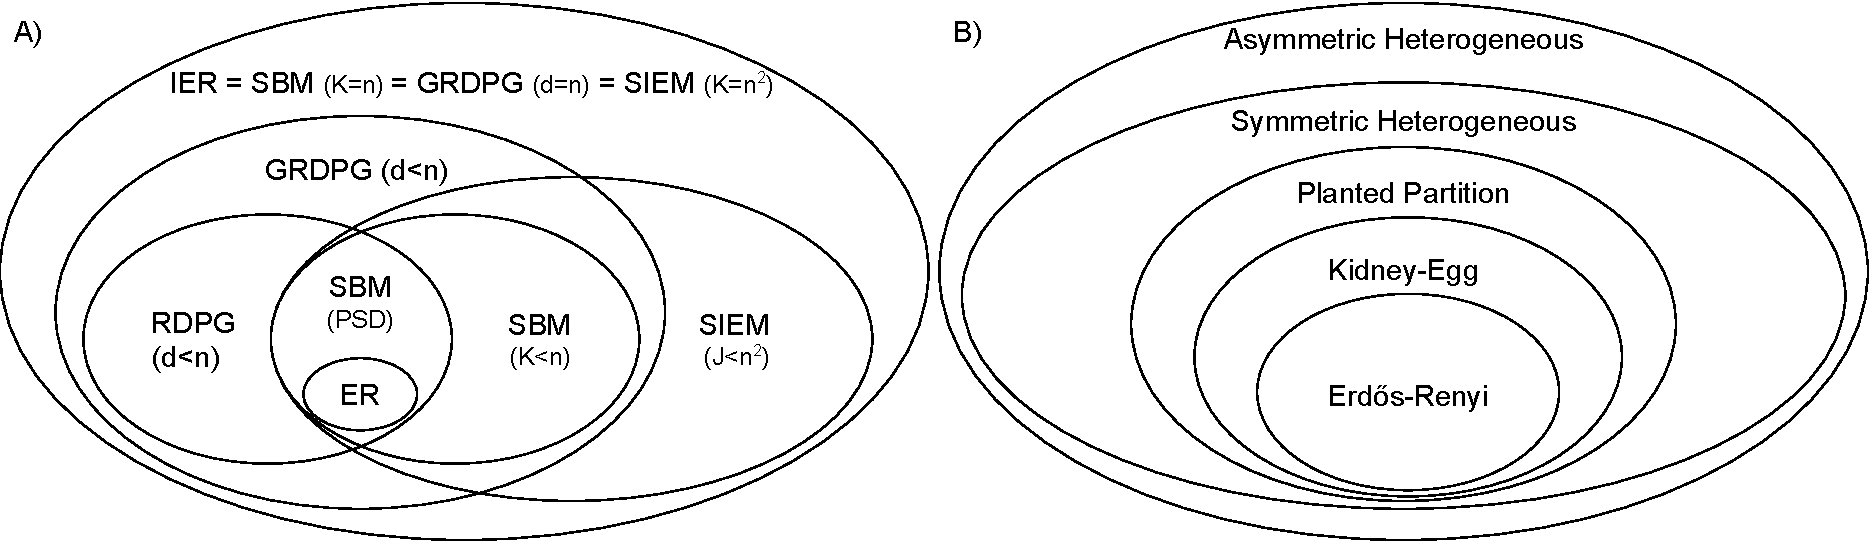
\includegraphics[width=\textwidth]{figures/dnd/models_combined}
    \caption{\textbf{Hierarchical Relationships of Statistical Models} 
    \textbf{(a)} Relationships among all the single-graph statistical models. Erd\H os-R\'enyi ($\er$) model is a stochastic block model ($\sbm$) with one community. $\sbm$ with a positive semidefinite block probability matrix $\B$ is also a random dot product graph ($\rdpg$). Any $\sbm$, $\rdpg$, and some structured independent edge model ($\siem$) can be represented as $d$-dimensional generalized random dot product graph ($\grdpg$) with $d$ less than number of vertices $n$. Inhomogenous Erd\H os-R\'enyi ($\ier$) model is equivalent to a $n$-block $\sbm$, $n$-dimensional $\grdpg$, and $n^2$-group $\siem$.
    \textbf{(b)} Relationships among the two-block $\sbm$ models. The most complex model is the asymmetric heterogeneous $\sbm$, and the simplest model is the $\er$, which is a degenerate case of 2-block $\sbm$.}
    \label{fig:models}
\end{figure}

\subsection{Single Graph Models}\label{sec:single_graph_models}
\subsubsection{Erd\H os-R\'enyi Random Graphs (ER)}\label{sec:uer}
The simplest random graph model is the $\mathsf{Erd\ddot{o}s-R\acute{e}nyi~(ER)}$ model \citep{Erdos1959-zf}. For a given set of $n$ vertices, each distinct pair of vertices are connected independently with probability $p \in [0, 1]$. Specifically, $\A \sim\er_n(p)$ if $\A$ has entries $\A_{ij}\sim\bern(p)$ for $i, j \in [n]$. While the $\er$ model is not representative of real data, it has been studied extensively since many of its properties can be solved exactly  \citep{newman2003random,Rukhin2010}.  

\subsubsection{Stochastic Block Model (SBM)}\label{sec:usbm}
First introduced in \cite{holland1983stochastic}, $\sbm$ is a model that can produce graphs with vertices grouped into $K$ communities \citep{Rohe2011-ha,sussman2012consistent,Wasserman1987-tw}. There are two simple variations of the $\sbm$ in which the vertex assignment vector $\vec \tau \in \left\{1, \hdots, K\right\}^n$ is known \textit{a priori}, and where $\vec \tau$ is not known. 
In both cases, a symmetric $K \times K$ block connectivity probability matrix $\B$ with entries in $[0,1]^{K \times K}$ governs the probability of an edge between vertices given their block memberships. 

If $\vec \tau \in \left\{1, \hdots, K\right\}^n$ is known \textit{a priori}, the \textit{a priori} $\sbm$ is parametrized only by the block connectivity matrix $\B$, and the model is $\A \sim \sbm_n(\vec \tau,\B)$ if $\A$ has entries $\A_{ij} \sim \bern(\B_{kl})$ where $\tau_i = k, \tau_j = l$, for $i, j \in [n]$, and $k, l \in [K]$. In the case where $\vec \tau$ is not known, the \textit{a posteriori} $\sbm$ is additionally parameterized by a block membership probability vector $\vec{\pi} = [\pi_1,\dots,\pi_K]^\top$ on the probability simplex.
The model is $\A \sim \sbm_n(\vec \pi,\B)$ if $\A$ has entries $\A_{ij} \big | k=\tau_i, l=\tau_j \sim \bern(\B_{kl})$, where $\tau_i {\sim} \multinomial(\vec \pi)$ for $i = 1, \hdots, n$. 

Throughout the context of this paper, we will focus particularly on a few variations of the two-block $\sbm$ ($K=2$) with block connectivity matrix $\B = \begin{bmatrix}a & b \\ c & d \end{bmatrix}$, abbreviated as $\B = [a, b; c, d]$. The common variants include:
\begin{enumerate}
    \item $\mathsf{Kidney-Egg}$: $b = c = d$. In this model, one of the blocks has edges with a different probability than the others, but the remaining blocks are homogeneous, where $a \neq b$. Furthermore, when $b > a$, the model is referred to as core-periphery $\sbm$.
    \item $\mathsf{Planted~Partition}$: $a = d$ and $b = c$. In this model, the within-block edges share a common probability $a$, and the between-block edges share a common probability $b$, where $a \neq b$.
    \item $\mathsf{Symmetric~ Heterogeneous}$: $b = c$. In this model, the between-block edges share a common probability $b$, but the within-block edges have a disparate probabilities, where $a \neq b \neq d$. 
    \item $\mathsf{Asymmetric~ Heterogeneous}$: $a \neq b \neq c \neq d$. In this directed model, every block has a unique probability.
    \item $\mathsf{Erd\ddot{o}s-R\acute{e}nyi}$: $a=b=c=d$. In this degenerate model, all blocks have a common probability, and the partitioning is irrelevant. 
    \item $\mathsf{Homophilic/Assortative/Affinity}$: $a, d > b, c$. In this model, the within-block probabilities are greater than cross-block probabilities.
    \item $\mathsf{Disassortative}$: $ b, c > a, d$. In this model, the cross-block probabilities are greater than the within-block probabilities.
\end{enumerate}
Figure \ref{fig:models}b summarizes the relationships of $\sbm$ models.

\subsubsection{Structured Independent Edge Model (SIEM)}\label{sec:usiem}
$\siem$ is a generalization of $\sbm$ that produces graphs in which edges are grouped into one of $K$ clusters. Analogous to the vertex assignment vector of the \textit{a priori} $\sbm$, the $\siem$ features an edge community assignment matrix $\M \in \left\{1, \hdots, K\right\}^{n \times n}$ which is known \textit{a priori}. Given the community assignment matrix $\M$, the $\siem$ is $\A \sim \siem_n(\M, \vec p)$ if $\A_{ij} {\sim}\bern(p_k)$ where $\M_{ij} = k$, for $i, j \in [n]$ and $k \in [K]$. $\vec p = [p_1, \hdots, p_K]^\top \in [0, 1]^K$ is the edge probability vector which governs the probability of an edge between vertices. 

The \textit{a priori} $\sbm$ is a special case of $\siem$ in which edges are assigned to blocks $\M$ which respect the vertex assignment vector $\vec \tau$. For the purposes of this paper, we will consider a case that frequently comes up in neuroimaging, the $\mathsf{Homotopic~ SIEM}$, in which each vertex has a matched ``pair'' amongst other vertices. The edges corresponding to a pair $\M_{ij} = 2$ where $(v_i, v_j)$ are a pair of vertices sharing a property, and the edges corresponding to a non-pair are $\M_{ij} = 1$. A matched pair of vertices, for instance, could be homotopic brain regions (two brain regions with similar function but in opposing hemispheres of the brain).

\subsubsection{Random Dot Product Graphs (RDPG)}\label{sec:rdpg}
$\rdpg$ belongs to the class of latent position random graphs \citep{hoff2002latent}. In a latent position graph, every vertex has associated to it a (typically unobserved) \textit{latent position} in some space $\mathcal{X}$, and the probability of connection between vertices $i$ and $j$ are given by a link function. In $\rdpg$, the space $\mathcal{X}$ is a constrained subspace of Euclidean space $\RR^d$ and the link function is the dot product \citep{Young2007-vu,scheinerman2010modeling,Sussman2014-zq}. Thus, in a $d-$dimensional $\rdpg$ with $n$ vertices, the matrix $\X\in \RR^{n\times d}$ whose rows are the latent positions, and the matrix of connection probabilities is given by $\Pbf=\X\X^\top$, which is positive semidefinite. The model is $\A\sim \rdpg_n(\X)$ if the adjacency matrix $\A$ has entries $\A_{ij} \sim \bern(\X_i\X_j^\top)$.
Subsequent inference tasks include community detection \cite{sussman2012consistent}, vertex classification \cite{tang2013}, or two-sample hypothesis testing for graphs with matched and non-matched vertices for a pair of graphs  \citep{priebe2019two,tang2017nonparametric,tang2017semiparametric}.

The $\rdpg$ is a flexible model, and other models of interest can be seen as special cases of the $\rdpg$. A $\sbm$ whose block connectivity matrix $\B$ is positive semi-definite is a $\rdpg$ with $K$ distinct latent positions. Thus, a $\sbm$ with $K$ blocks can be represented with a latent position matrix $\X\in\RR^{n\times d}$, with $d\leq K$, where there are only $K$ different rows of $\X$, and letting $\X_{\mathcal{U}}\in\RR^{K\times d}$ be the matrix with the subset of the rows $\mathcal{U}$ where each row is the latent position for a block, then the block connectivity matrix is $\B= \X_\mathcal{U}\X_\mathcal{U}^\top \in\RR^{K\times K}$. More generally, the $\rdpg$ can represent other models with more complex structures, such as mixed memberships \citep{Airoldi2008-tp} or hierarchical communities \citep{Lyzinski2017-cq}.

\subsubsection{Generalized Random Dot Product Graphs (GRDPG)}\label{sec:grdpg}
Unlike $\rdpg$ model, $\grdpg$ does not assume that $\Pbf$ is a positive semidefinite probability matrix  \citep{rubin2017statistical}. In this model, the edge probability matrix is given by $\Pbf=\X \I_{pq}\X^\top$, and $\A\sim\grdpg_n(
\X, p, q)$ if $\A_{ij}\sim\bern(\X_i\I_{pq}\X_j^\top)$ where $\I_{pq}=\textrm{diag}(1, \ldots, 1, -1, \ldots, -1)$  with $p$ ones followed by $q$ minus ones on its diagonal, and where $p \geq 1$ and $q \geq 0$ are two integers satisfying $p + q = d$.

The $\grdpg$ generalizes all of the previous models. When $q=0$, $\grdpg$ reduces to a $\rdpg$ model. To represent any $\sbm$ as $\grdpg$, let $p\geq 1, q\geq 0$ be the number of positive and negative eigenvalues of the block connectivity matrix $\B\in\RR^{K\times K}$, respectively. The block matrix can be represented as $\B = \X_\mathcal{U}\I_{pq}\X_\mathcal{U}^\top$.


\subsubsection{Inhomogenous Erd\H os-R\'enyi Random Graphs (IER)}\label{sec:uierrg}
The $\mathsf{Inhomogenous~Erd\ddot{o}s-R\acute{e}nyi~(IER)}$ is a model where each pair of nodes has a unique probability of an edge existing between the two, and is therefore the most general independent edge model. For a given set of $n$ vertices, the $\ier$ is parametrized by a matrix $\Pbf \in [0, 1]^{n \times n}$, where $\Pbf_{ij}$ is the probability of an edge connecting vertices $v_i, v_j$ where $i, j \in [n]$. That is, $\A \sim \ier_n(\Pbf)$ if $\A$ has entries $\A_{ij}\sim \bern(\Pbf_{ij})$ for $i, j \in [n]$. $\ier$ cannot be estimated from a single graph, as there are $n\choose 2$ unknowns (the probabilities) with $n\choose 2$ total observations (the edges).

Note that all single graph models are special cases of $\ier$. Additionally, $\sbm$ with $K=n$, $\siem$ with $K=n^2$, and $\grdpg$ with $d=n$ are equivalent to an $\ier$ model.

\subsection{Multiple Graph Models}\label{sec:multi_graph_models}

A common idea in statistical models for multiple graphs is a shared latent space that contain structural information common to all graphs. The two models presented in this section constrain the shared latent space in different ways to describe the heterogeneity in graphs, which results in sensitivity to different kinds of heterogeneity. The advantages and disadvantages of each model are highlighted in Section \ref{sec:multi_app}.

In the following models, consider a sample of $m$ observed graphs $\mathcal{G}^{(1)}, \mathcal{G}^{(2)}, \ldots, \mathcal{G}^{(m)}$  and their associated adjacency matrices, $\A^{(1)}, \A^{(2)}, \ldots, \A^{(m)}\in\RR^{n\times n}$ with $n$ vertices that are identical and shared across all graphs. 

\subsubsection{Joint Random Dot Product Graphs (JRDPG)}
In this model, we consider a collection of $m$ $\rdpg$s all with the same generating latent positions. Similar to a $\rdpg$, given an appropriately constrained Euclidean subspace $\RR^d$, the model is parameterized by a latent positions matrix $\X\in\RR^{n\times d}$ where $d \ll n$. The model is $\left(\A^{(1)}, \A^{(2)}, \ldots, \A^{(m)}\right)\sim \jrdpg(\X)$ where $\A_{ij}^{(l)}\sim \bern(\X_i\X_j^\top)$ for all $i, j \in [n]$ and $l\in [m]$. Each graph has marginal distribution $\A^{(l)}\sim\rdpg(\X)$ for all $l \in [m]$, meaning that the matrices $\A^{(1)}, \ldots,\A^{(m)}$ are conditionally independent given $\X$ \citep{athreya2017statistical,levin2017central}. While the model assumes that the latent positions for the graphs are the same, we note that this assumption is likely violated in heterogeneous networks, but still remains a very useful model as shown in Section \ref{sec:multi_app}.

\subsubsection{Common Subspace Independent-Edge Model (COSIE)} \label{sec:cosie}
In this model, the heterogeneous networks are described via a shared latent structure on the vertices, but also permits sufficient heterogeneity via individual matrices for each graph  \citep{arroyo2019inference}.
The model is parameterized by a  matrix $\V\in\RR^{n\times d}$ with orthonormal columns, 
where $n$ is the number of vertices and $d\ll n$, and  symmetric individual score matrices $\R^{(i)}\in\RR^{d\times d}$. The matrix $\V$ characterizes a low-rank common subspace, and is related to the latent positions for the vertices, and the score matrices incorporate individual differences to model the heterogeneity of the graphs. The model is denoted by $\left(\A^{(1)}, \ldots, \A^{(m)}\right)\sim \cosie(\V; \R^{(1)}, \ldots, \R^{(m)})$ where $\A_{ij}^{(l)} \sim \bern(\mathbf{P}^{(l)}_{ij})$ for all $i, j\in [n], i < j$, and $\mathbf{P}^{(l)}=\V\R^{(l)}\V^\top$. This factorization of the expected adjacency matrices is related to other decompositions for multiple matrices into population singular vectors or eigenvectors and individual parameters \citep{afshin2012enhancing,crainiceanu2011population,lock2013joint,wang2019common}.


\subsubsection{Correlated Models} \label{sec:correlated-graphs}


Finally, we are interested in graph models for a pair of graphs, $\mathcal{G}_1$ and $\mathcal{G}_2$, where the two graphs are said to be correlated; that is, the edges adjoining incident vertices have a non-zero correlation. Correlated graph models have numerous applications, such as when a graph is estimated repeatedly for the same source at different points in time.

\paragraph{Correlated $(\Pbf,\Q)$}
The $\mathbf{R}$-correlated $(\Pbf, \Q)$ model \citep{lyzinski2017matchability} with parameters $\mathbf{R}, \Pbf, \Q\in[0,1]^{n\times n}$, denoted as $\mathrm{CorrER}(\Pbf, \Q, \mathbf{R})$, produces two graphs $\mathcal{G}_1$ and $\mathcal{G}_2$ with adjacency matrices $\A^{(1)}, \A^{(2)}$ such that each graph is marginally an inhomogeneous Erd\H{o}s-R\'enyi with $\A^{(1)} \sim \ier(\Pbf)$, $\A^{(2)}\sim \ier(\Q)$, but the  pairs of corresponding edges have Pearson correlation  encoded in the matrix $\mathbf{R}$ such that 
$$\mathbf{R}_{ij} = \text{Corr}(\A^{(1)}, \A^{(2)})= \frac{\mathbb{P}(\A^{(1)}_{ij}=\A^{(2)}_{ij}=1)-\Pbf_{ij}\Q_{ij}}{\sqrt{\Pbf_{ij}(1-\Pbf_{ij}) \Q_{ij}(1-\Q_{ij})}}.$$
When $\Pbf$ and $\Q$ are different, there are restrictions in the values that the correlation matrix $\mathbf{R}$ can take. In particular, if $\Pbf_{ij}\neq\Q_{ij}$  and $\Pbf>\Q$, then $\mathbf{R}_{ij}\leq \sqrt{\frac{\Q_{ij}(1-\Q_{ij})}{\Pbf_{ij}(1-\Pbf_{ij})}}$ \citep{lyzinski2017matchability}.


We are interested particularly in two special cases of the $\mathrm{CorrER}(\Pbf, \pmb Q, \pmb R)$:
\begin{enumerate}
    \item The $\rho$-correlated $\rdpg$ model arises when $\Pbf = \Q=\X\X^\top$ for some latent position matrix $\X \in \RR^{n \times d}$  as in Section \ref{sec:rdpg}, and $\pmb R = \rho \pmb 1_{n \times n}$ (that is, the matrix of edge correlations $\pmb R$ has only a single unique entry $\rho\geq 0$). We say that $\A_1, \A_2 \sim \rho\rdpg(\X)$.
    \item The $\rho$-correlated $\er$ model arises in the case where $\Pbf = \Q = p\pmb 1_{n \times n}$ (i.e.,  the probability matrix has a single unique entry $p>0$), and $\pmb R = \rho\pmb 1_{n \times n}$ (as above, the matrix of correlations has a single unique entry). We say that $\A_1, \A_2 \sim \rho\er(p)$.
\end{enumerate}